\section{Architektura IoT sítí}
  V blízké době se očekává stále větší nárůst zařízení, která jsou připojena k internetu.
  Dle odhadů by jejich počet měl v roce 2020 překročit 30 miliard \cite{iotDevices}.
  Pro takové množtví připojení už není možné, aby každé zařízení komunikovalo přímo
  se vzdáleným datovým centrem, protože nároky na potřebnou šířku pásma by byly 
  obrovské \cite{fog}.
  Dalším problémem je často velmi omezený výkon připojených prvků, který je nezbytný pro 
  použití bezpečnostních funkcí umožňujících kompletně zabezpezpečenou komunikaci. 
  
  Řešení těchto problémů je do probíhající komunikace přidat několik podvrstev, 
  které umožní přesunout výpočetní výkon blíže ke koncovým zařízením, a tím celý
  proces zpracování dat provést efektivněji.
 \subsection{Fog computing} 
 Fog computing je rozšíření Cloud computingu, které spočívá v přesunutí výpočetního
 výkonu blíže k okraji sítě. Rozšíření je umožněno pomocí přidání síťových zařízení,
 které kromě síťových funkcionalit nabízí i výpočetní výkon pro běh programů. Programy 
 je často možné nasadit pomocí konterjnerů nebo samostatných virtuálních strojů, což 
 velmi usnadňuje jejich distribuci \cite{fog}.
 
 Porovnání klasické a Fog architektury se nachází na obrázku \ref{obr.fog}. V reálném nasazení může
 být použito i více Fog vrstev, kde každá provádí určitý stupeň předzpracování a řízení
 dat.
\begin{figure}[ht]
\begin{center}
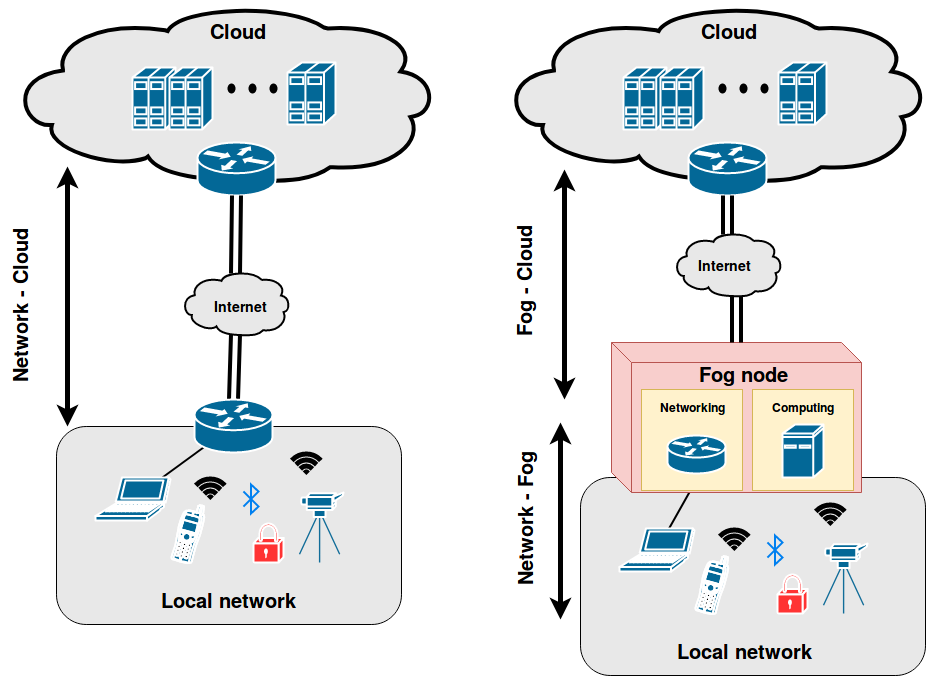
\includegraphics[scale=0.38]{pictures/fog}
\caption{Porovnání klasické a Fog architektury}
\label{obr.fog}
\end{center}
\end{figure}
 Zavedením principů Fog computingu vznikají pro síť následující výhody:
 \begin{itemize}
 \item \textbf{Zlepšení bezpečnosti} \cite{fog}
 
     Síťové prvky jsou trvale napájené a připojené k internetu. Podporují pokročilé
     bezpečnostní funkce, a proto je možné například vytvářet šifrované tunelové
     spojení pro bezpečný přenos dat.     
\item \textbf{Nižší nároky na šířku pásma a latency} \cite{fog}

    Odeslaná data z koncových zařízení jsou zpracovávána a filtrována na okraji 
    sítě. Tím je možné rychleji reagovat na přijaté zprávy a snížit nároky
    na latency a šířku pásma. Zároveň krátkodobá data mohou být uložené ve 
    Fog vrstvě a centrální datové cetrum může být využito pro dlouhodobé údaje, 
    které se zpracovávají pokročilými algoritmy pro analýzu dat.
 \item \textbf{Jednotná správa} \cite{fog}
 
    Při správě sítě už se nemusí přistupovat přímo na koncové prvky, které 
    často komunikují různými protokoly, ale stačí pouze
    řídit síťová zařízení v jednotlivých Fog vrstvách, které odstiňují různorodost
    protokolů a nabízí standardizovaný přístup. Díky této abstrakci je 
    zároveň zjednodušeno zpracování získaných dat a je umožněno přímé zasílání zpráv
    mezi koncovými prvky, které používají odlišné komunikační protokoly.
 \end{itemize} 
 
 \subsection{IoT brána} 
 IoT brána je síťové zařízení, které je umístěno velmi blízko koncových zařízení
 a představuje vstup do Fogové vrstvy. Jejím hlavním cílem je získávat data 
 z připojených zařízení a poskytovat je vyšším vrstvám. Pokud je brána reprezentována
 výkonnějším síťovým prvkem, tak v rámci brány může probíhat i základní zpracování
 dat. 
 
 Pro IoT sítě je typické, že obsahují velké množtví koncových prvků komunikujících
 různorodými způsoby. Zejména senzory použivají protokoly, které nepodporují
 IP (Internet Protocol) spojení. Důvodem použití této komunikace je často velký
 důraz na nízkou spotřebu a specifické požadavky na způsob zasílání zpráv.
 Příkladem protokolů pro senzorové sítě ne například:
 Z-Wave, Bluetooth a Zigbee. Jejich detailní popis se nachází v kapitole \ref{senzory}.
 Tato různorodost vyžaduje od brány, aby obsahovalo dodatečná rozhranní, které 
 umožní připojení nejrůznějších bezdrátových i drátových koncových prvků.
 \subsection{Komunikační model a jeho hrozby}
 Při použití principů popsaných v předchzích kapitolách lze model komunikace
 do následujících vrstev \cite{iotSurvey}:
 \begin{itemize}
 \item Aplikační vrstva 
 \item Síťová vrstva
 \item Senzorová vrstva
\end{itemize}
 Jednotlivé vrstvy budou popsány v následujích podkapitolách.
 
 \subsubsection{Senzorová vrstva}
 \subsubsection{Síťová vrstva}
 \subsubsection{Aplikační vrstva}
 
 \section{Analýza síťových protokolů}
 % popis funkce fungování MQTT, COAP, (AMQP)
 \section{Analýza senzorových protokolů} \label{senzory}
 % popis a bezpečnostní analýza ZWave a Bluetooth
 \section{Způsoby obrany}
 % popis IDS principů
 \section{BeeeOn brána}
 \section{NEMEA framework}
 \section{Existující řešení}
 % aktuální řešení funguje na cetrálním monitorovacím prvku, které monitoruje IP
 % teprve nedávno vznikly signatury pro SCADA
 \section{Analýza požadavků}
 \section{Zvolené řešení}
